\documentclass[11pt,a4paper]{report}
\usepackage[utf8]{inputenc}
\usepackage{amsmath}
\usepackage{graphicx}
\usepackage{geometry}
\geometry{margin=1in}
\usepackage{hyperref}

\title{McCann model for rhomohedral graphene}
\date{\today}

\begin{document}

\maketitle

\chapter{Anomalous Hall Effect}

\section{Introduction}
This report analyzes the behavior of ABC-stacked multilayer graphene using the McCann model. We specifically compare the cases for $N=1$ (monolayer) and $N=5$ layers, focusing on their energy bands, Berry curvature, and the convergence of the local Chern number contribution.

\section{Model and Analytical Equations}
The system is described by a 2x2 effective Hamiltonian in the vicinity of a K point (low energy):
\begin{equation}
H = \begin{pmatrix}
\Delta & X(\mathbf{k}) \\
X^\dagger(\mathbf{k}) & -\Delta
\end{pmatrix}
\end{equation}
where $2\Delta$ is the energy gap and $X(\mathbf{k})$ is the off-diagonal coupling term. In polar coordinates $(k, \phi)$, the term $X$ for $N$ layers is given by:
\begin{equation}
X(k, \phi) = \frac{(v k e^{i \xi \phi})^N}{(-\gamma_1)^{N-1}}
\end{equation}
where $v = \frac{\sqrt{3}}{2} \gamma_0$ in natural units ($a=1$, $\hbar=1$) and $\xi = \pm 1$ is the valley index.

\subsection{Energy Bands}
The eigenvalues of the Hamiltonian represent the energy bands:
\begin{equation}
\varepsilon(\mathbf{k}) = \pm E(\mathbf{k}) = \pm \sqrt{|X(\mathbf{k})|^2 + \Delta^2}
\end{equation}

\subsection{Eigenstates}
The normalized eigenstates for the positive and negative bands are given by:
\begin{equation}
|\psi_+\rangle = \frac{1}{\mathcal{N}_+} \begin{pmatrix} E + \Delta \\ X^\dagger \end{pmatrix}, \quad 
|\psi_-\rangle = \frac{1}{\mathcal{N}_-} \begin{pmatrix} -X \\ E + \Delta \end{pmatrix}
\end{equation}
where $\mathcal{N}_{\pm}$ are the normalization constants.

\subsection{Berry Curvature}
The Berry curvature $\Omega$ is calculated using the Kubo-like formula. For the results presented in this report, we specifically show the Berry curvature calculated for the positive energy band:
\begin{equation}
\Omega_n = i \sum_{m\neq n} \frac{\langle \psi_{n} | \mathbf{\nabla_k} H | \psi_{m} \rangle \times \langle \psi_{m} | \mathbf{\nabla_k} H | \psi_{n} \rangle}{(E_{n} - E_{m})^2}
\end{equation}
Here, the gradient is calculated in polar coordinates as:
\begin{equation}
    \mathbf{\nabla_k} = \frac{\partial}{\partial k}\vec{e}_k + \frac{1}{k} \frac{\partial}{\partial \phi} \vec{e}_{\phi}
\end{equation}

\section{Numerical Results}

\subsection{Energy Bands Comparison}
Figure \ref{fig:bands} shows the energy bands for $N=1$ and $N=5$. For $N=1$, the dispersion is linear at high $k$ (Dirac-like), while for $N=5$ it is much flatter near $k=0$ due to the $k^N$ dependence.

\begin{figure}[h]
    \centering
    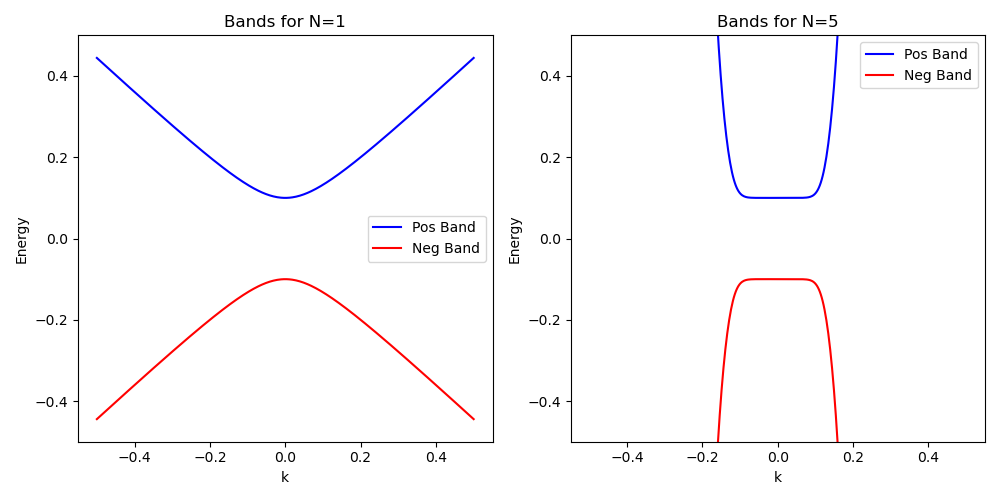
\includegraphics[width=0.8\textwidth]{../figures/bands_comparison.png}
    \caption{Energy bands for N=1 and N=5 layers.}
    \label{fig:bands}
\end{figure}

\subsection{Berry Curvature}
The Berry curvature for $N=1$ peaks sharply at $k=0$. However, for $N=5$, the curvature is suppressed at the center and peaks at finite $k$ (Figure \ref{fig:berry}).

\begin{figure}[h]
    \centering
    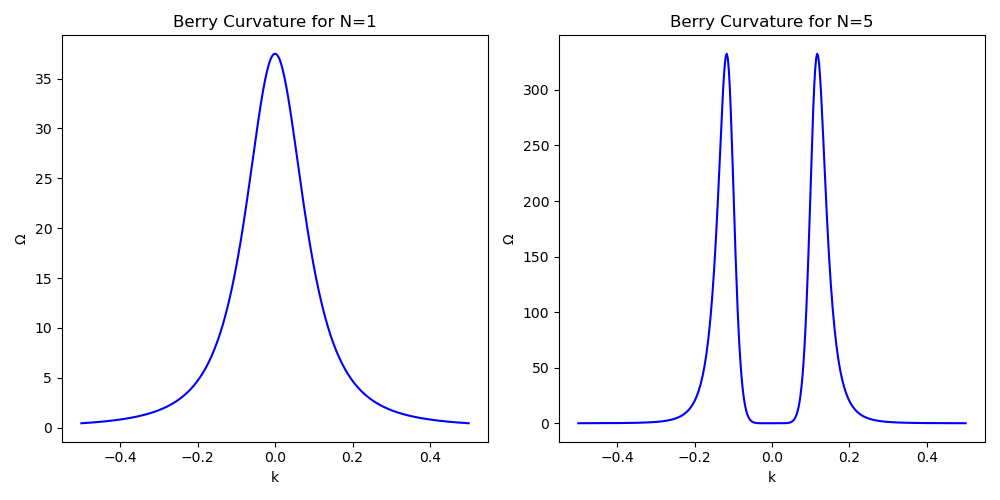
\includegraphics[width=0.8\textwidth]{../figures/berry_curv_comparison.png}
    \caption{Berry curvature comparison (Positive Band).}
    \label{fig:berry}
\end{figure}

\section{Berry Curvature Integration}

The local Chern number contribution is obtained by integrating the Berry curvature over a region in $k$-space. While the McCann model is isotropic and naturally expressed in polar coordinates, the numerical integration is performed over a uniform Cartesian meshgrid $(k_x, k_y)$. This choice provides several numerical advantages:
\begin{itemize}
    \item \textbf{Uniform Sampling Density:} In a Cartesian grid, every point represents an identical area element $\Delta A = \Delta k_x \Delta k_y$. In a polar grid, the area element $dA = k \, dk \, d\phi$ is proportional to $k$ and vanishes as $k \to 0$. Since the Berry curvature is often highly concentrated near the Dirac point ($k=0$ for monolayer graphene), the Cartesian grid ensures high sampling density where it is most needed without requiring a non-linear radial distribution.
    \item \textbf{Singularity Avoidance:} The Cartesian coordinate system avoids the coordinate singularity at the origin inherent to polar grids, which simplifies the handling of the peak in $\Omega$ at $k=0$ for $N=1$.
    % \item \textbf{Simplified Masking:} Evaluating the integral over an arbitrary region (such as an energy-restricted domain) becomes a straightforward summation over masked points in the flattened grid.
\end{itemize}

To ensure a consistent comparison between different layer numbers $N$, we define the integration domain using an energy cutoff $E_{max}$ rather than a fixed momentum radius. The integral is evaluated numerically as:
\begin{equation}
C_{local}(E_{max}) = \frac{1}{2\pi} \iint_{E(\mathbf{k}) \le E_{max}} \Omega_{pos}(\mathbf{k}) dk_x dk_y \approx \frac{\Delta A}{2\pi} \sum_{i \in \text{mask}} \Omega_{pos}(\mathbf{k}_i)
\end{equation}
where the sum runs over all points $k_i$ satisfying the energy condition $E(\mathbf{k}_i) \le E_{max}$, and $\Delta A$ is the constant area per grid point.

Figure \ref{fig:convergence} shows that as the energy cutoff $E_{max}$ increases, the integral converges to $N/2$.

\begin{figure}[h]
    \centering
    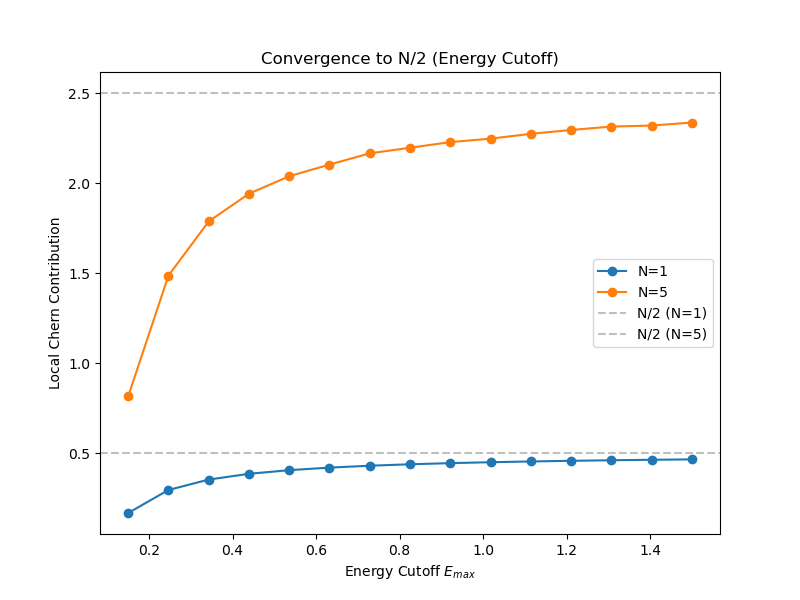
\includegraphics[width=0.65\textwidth]{../figures/chern_convergence.png}
    \caption{Convergence of the local Chern number contribution to $N/2$ as a function of the energy cutoff $E_{max}$.}
    \label{fig:convergence}
\end{figure}


\section{Valley Comparison}
The two K-valleys in the hexagonal lattice, indexed by $\xi = \pm 1$, are related by time-reversal symmetry. While the energy dispersion is identical for both valleys, the Berry curvature of a given band changes its sign:
\begin{align}
    \mathcal{T}:~~ &\mathbf{k} \to -\mathbf{k}\\
        &E(\mathbf{-k}) = E(\mathbf{k}) \notag \\
        &\Omega(-\mathbf{k}) = -\Omega(\mathbf{k}) \notag
\end{align}
Figure \ref{fig:valley_comp} compares the positive energy band and the corresponding Berry curvature for $N=5$ layers, showing the sign inversion between the two K valleys.

\begin{figure}[h]
    \centering
    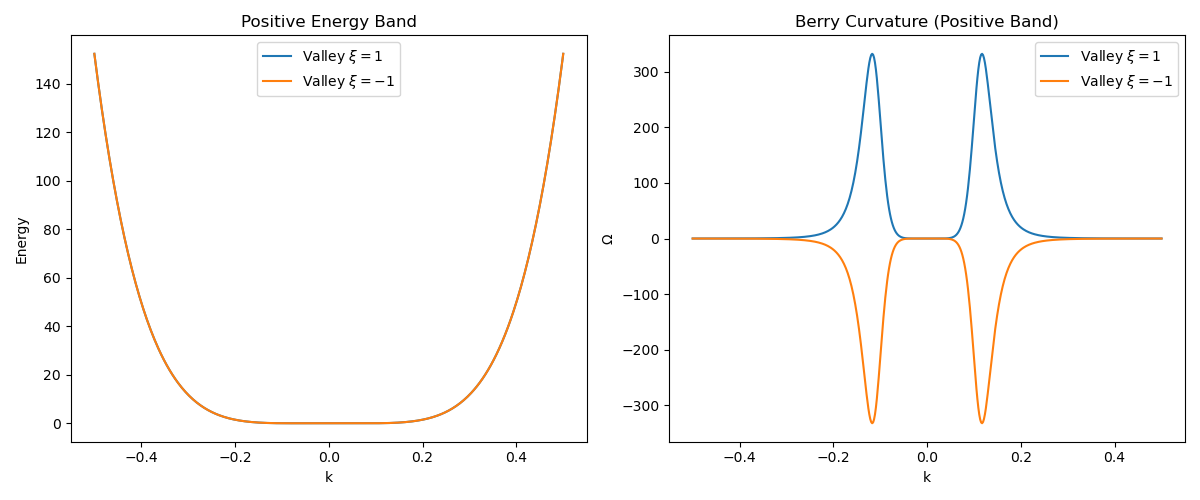
\includegraphics[width=1.0\textwidth]{../figures/valley_comparison_detailed.png}
    \caption{Comparison of the positive energy band (left) and Berry curvature (right) for valleys $\xi=1$ and $\xi=-1$ ($N=5$ layers).}
    \label{fig:valley_comp}
    \end{figure}

Consequently, the local Chern number contributions for $N=5$ have opposite signs. The integration of the Berry curvature over a circle of radius k=1 gives:
\begin{itemize}
    \item Valley $\xi = 1$: $C_{local} = 2.499949$
    \item Valley $\xi = -1$: $C_{local} = -2.499949$
\end{itemize}
The total Chern number for the system, considering both valleys, would vanish in the presence of time-reversal symmetry ($C_{tot} = C_{K} + C_{K'} = 0$).

\section{Anomalous Hall Effect with Spin}

Recent additions to the project include the calculation of the Anomalous Hall Effect (AHE) considering both spin and valley degrees of freedom.

\subsection{Magnetic AHE at $\mu=0$}
We calculate the total Hall conductivity $\sigma_{xy}$ for the system at the Fermi level $\mu=0$. We use $N=5$ layers and a temperature $T=20$ K. The gap parameters used are:
\begin{itemize}
    \item Valley $K$ ($\xi=1$): $\Delta_{\uparrow} = 0.1$, $\Delta_{\downarrow} = 0.0$
    \item Valley $K'$ ($\xi=-1$): $\Delta_{\uparrow} = 0.0$, $\Delta_{\downarrow} = -0.1$
\end{itemize}

The calculated total conductivity for the spin-valley case (without SOC) is:
\begin{equation}
    \sigma_{xy}^{total}(\mu=0) \approx -5.000 \,\, e^2/h
\end{equation}
which corresponds to the sum of the Chern contributions of the occupied bands ($N/2 = 2.5$ per valley per spin when applicable).

\subsection{AHE vs. Chemical Potential}
The dependence of the AHE on the chemical potential $\mu$ was scanned using the following parameters:
\begin{itemize}
    \item Valley $K$: $\Delta_{\uparrow} = 0.1$, $\Delta_{\downarrow} = 0.0$
    \item Valley $K'$: $\Delta_{\uparrow} = 0.0$, $\Delta_{\downarrow} = -0.2$
\end{itemize}

Figure \ref{fig:ahe_scan} shows the results of the scan. It is important to note that the convergence to $0$ far from $\mu=0$ (as well as the convergence to $N/2$ when there is a plateau) is very slow and difficult to fully observe in numerical simulations due to the long tails of the Berry curvature.

\begin{figure}[h]
    \centering
    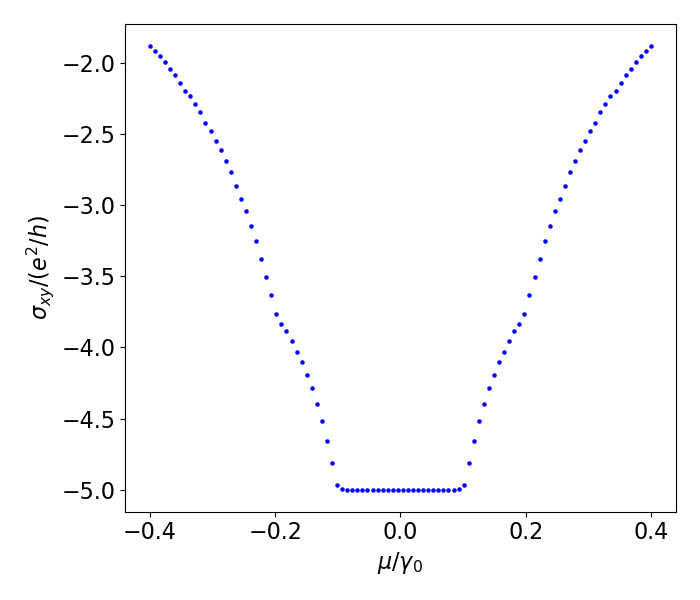
\includegraphics[width=0.7\textwidth]{../figures/ahe_scan_spinSOC.png}
    \caption{Total Hall conductivity $\sigma_{xy}$ as a function of the chemical potential $\mu/\gamma_0$ including spin and SOC.}
    \label{fig:ahe_scan}
\end{figure}

\chapter{NonLinear AHE and positional shift}

\section{Hamiltonian with Trigonal Warping}

In polar coordinates \((k, \phi) \in \left( [0, +\infty[, [0, 2\pi] \right)\), we define \(\pi = vke^{i\xi\phi}\).

\begin{equation}
    \mathcal{H}_{\xi, s} = \begin{pmatrix}
        \Delta_{\xi, s} & X(\pi) \\
        X^{\dagger}(\pi) & -\Delta_{\xi, s}
    \end{pmatrix}
\end{equation}

To introduce the trigonal warping, we expand \(X(\pi)\) to first order in perturbations (\(v_3, \gamma_2\)) with \(N = n_1 + 2n_2 +3n_3\), \(n_2\) being the order of \(v_3\) and \(n_3\) the order of \(\gamma_2\). \(X_0\) is the unpertrubed zero order term, then we write \(X_{n_2, n_3}\):

\begin{align}
    &X_0 = \frac{\pi^N}{(-\gamma_1)^{N-1}}\\
    X_{10} = (N-1)& \frac{v_3 \pi^{N-2} \pi^{\dagger}}{v(-\gamma_1)^{N-2}} = -\frac{4v_3v^3}{\gamma_1^3}k^4e^{i2\phi}\\
    X_{01} = \frac{(N-2)}{2}&\gamma_2 \left(\frac{\pi}{-\gamma_1}\right) = \frac{3v^2\gamma_2}{2\gamma_1^2}k^2e^{i2\phi}
\end{align}

\section{Nonlinear Conductivity}

For a given band:

\begin{equation}
    \sigma^{ijl} = \frac{\partial j_i}{\partial E_j \partial E_l} = \frac{e^3}{\hbar^2} \int \frac{d^2k}{(2\pi)^2} \frac{\partial f_n}{\partial \varepsilon_n} \left[ 2v_i G_{jl} - \frac{1}{2} \left(v_j G_{li} + v_l G_{ji}\right) \right]
\end{equation}

With the quantum metric for band 0 defined by:

\begin{equation}
    G_{ij} = 2\text{Re} \sum_{n \neq 0} \frac{(V_i)_{0n} (V_j)_{n0}}{(\varepsilon_0 - \varepsilon_n)^3}
\end{equation}

\section{Symmetry Constraints on the Conductivity}

\begin{itemize}
    \item \textbf{Mirror $\mathcal{M}_y\ (y \to -y)$:} components with an odd number of $y$ are 0.
    \item \textbf{$C_{3z}$ rotation:} only non-zero components are related: $\sigma_{xxx} = -\sigma_{xyy} = -\sigma_{yxy} = -\sigma_{yyx}$
\end{itemize}

\section{Evolution of Nonlinear Conductivity}

In this chapter, we analyze the behavior of the nonlinear conductivity $\sigma_{xxx}$ related to the positional shift. We focus on its dependence on the chemical potential $\mu$ for various gap configurations defined by the parameters $\Delta_{v,s}$, where $v \in \{K, K'\}$ and $s \in \{\uparrow, \downarrow\}$.

The plots below show the evolution of $\sigma_{xxx}$ for different scenarios of gap symmetries. The shaded regions represent the energy gaps for each spin and valley.

\subsection{Scenario A: Symmetric Gaps, Zero Minors}
Parameters: $\Delta_{K\uparrow}=0.1, \Delta_{K\downarrow}=0.0, \Delta_{K'\uparrow}=0.0, \Delta_{K'\downarrow}=-0.1$.
Here $\Delta_{1\uparrow} = -\Delta_{2\downarrow}$ and $\Delta_{1\downarrow} = \Delta_{2\uparrow} = 0$.

\begin{figure}[ht]
    \centering
    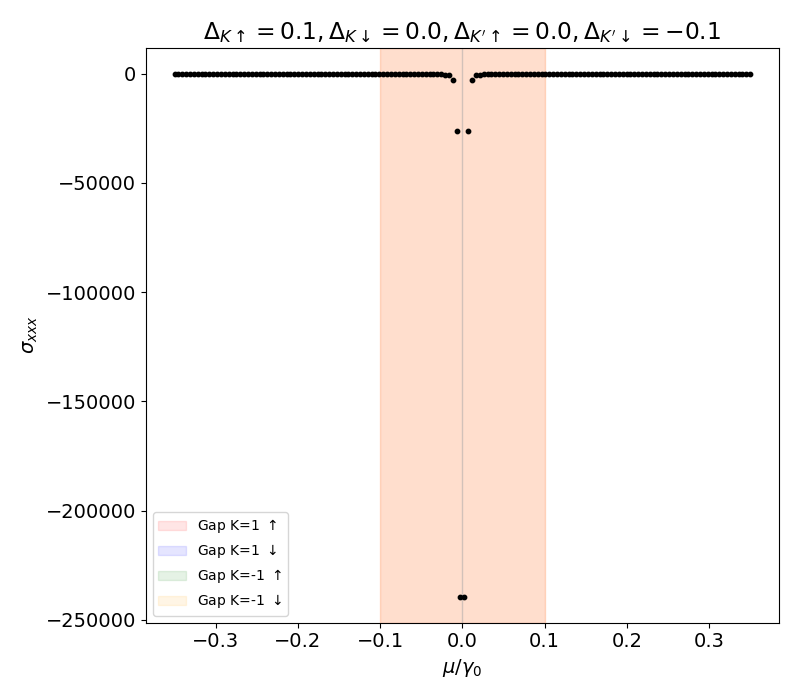
\includegraphics[width=0.6\textwidth]{../figures/scan_mu_PS_A.png}
    \caption{Nonlinear conductivity for symmetric gaps with zero minor gaps.}
    \label{fig:scan_A}
\end{figure}

\subsection{Scenario B: Symmetric Gaps, Non-Zero Minors}
Parameters: $\Delta_{K\uparrow}=0.1, \Delta_{K\downarrow}=0.05, \Delta_{K'\uparrow}=0.05, \Delta_{K'\downarrow}=-0.1$.
Here $\Delta_{1\uparrow} = -\Delta_{2\downarrow}$ and $\Delta_{1\downarrow} = \Delta_{2\uparrow} \neq 0$.

\begin{figure}[ht]
    \centering
    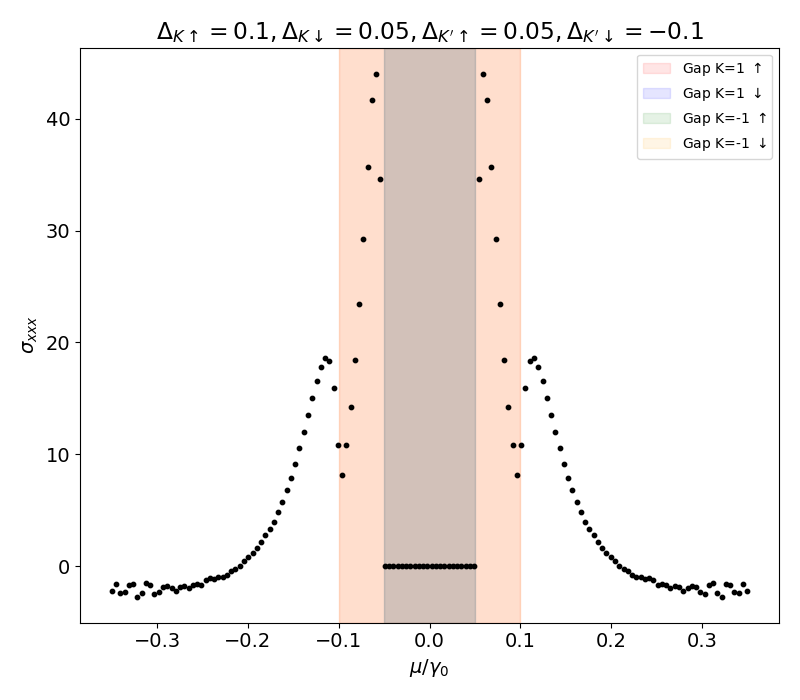
\includegraphics[width=0.6\textwidth]{../figures/scan_mu_PS_B.png}
    \caption{Nonlinear conductivity for symmetric gaps with non-zero minor gaps.}
    \label{fig:scan_B}
\end{figure}

\subsection{Scenario C: Asymmetric Gaps, Zero Minors}
Parameters: $\Delta_{K\uparrow}=0.1, \Delta_{K\downarrow}=0.0, \Delta_{K'\uparrow}=0.0, \Delta_{K'\downarrow}=-0.2$.
Here $\Delta_{1\uparrow} \neq -\Delta_{2\downarrow}$ and $\Delta_{1\downarrow} = \Delta_{2\uparrow} = 0$.

\begin{figure}[ht]
    \centering
    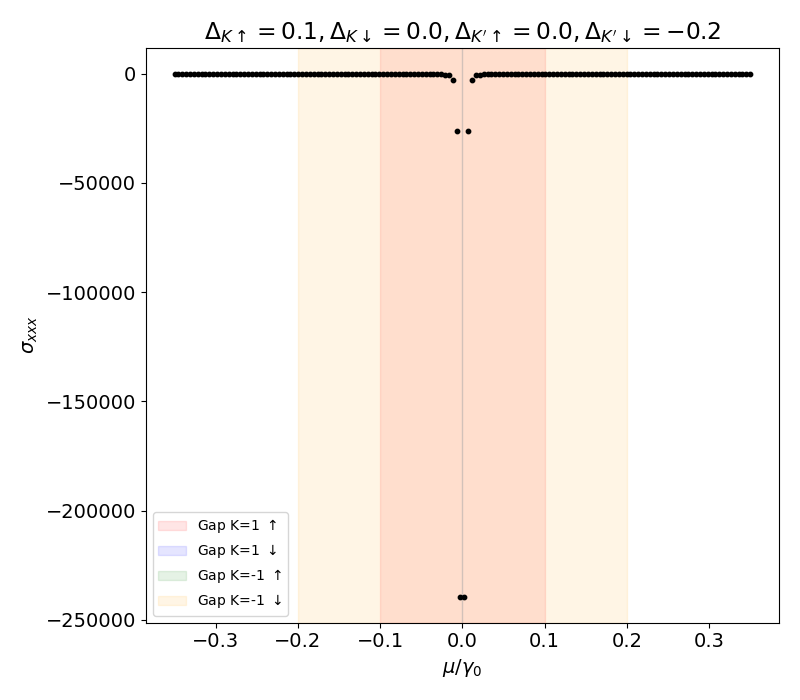
\includegraphics[width=0.6\textwidth]{../figures/scan_mu_PS_C.png}
    \caption{Nonlinear conductivity for asymmetric gaps with zero minor gaps.}
    \label{fig:scan_C}
\end{figure}

\subsection{Scenario D: Asymmetric Gaps, Non-Zero Minors}
Parameters: $\Delta_{K\uparrow}=0.1, \Delta_{K\downarrow}=0.05, \Delta_{K'\uparrow}=0.05, \Delta_{K'\downarrow}=-0.2$.
Here $\Delta_{1\uparrow} \neq -\Delta_{2\downarrow}$ and $\Delta_{1\downarrow} = \Delta_{2\uparrow} \neq 0$.

\begin{figure}[ht]
    \centering
    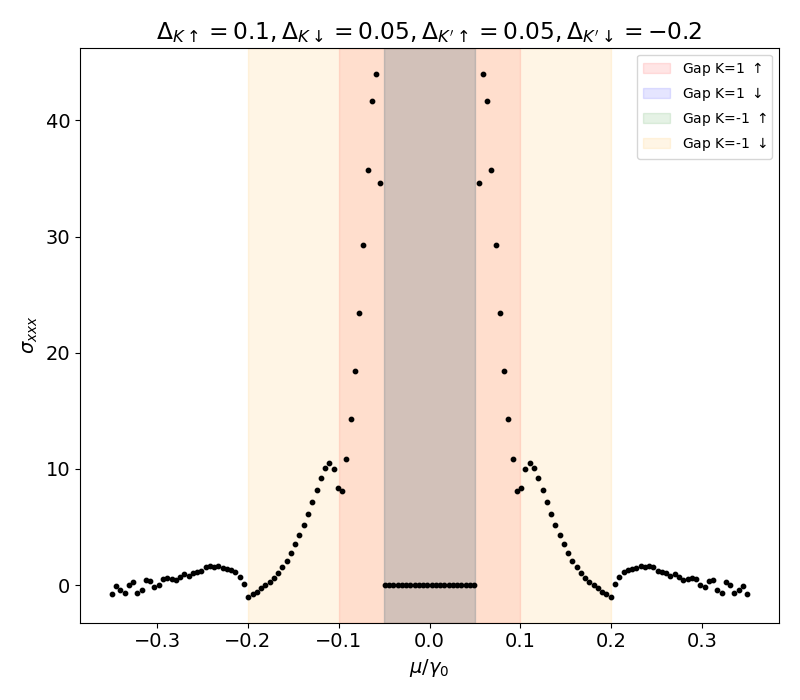
\includegraphics[width=0.6\textwidth]{../figures/scan_mu_PS_D.png}
    \caption{Nonlinear conductivity for asymmetric gaps with non-zero minor gaps.}
    \label{fig:scan_D}
\end{figure}

% \begin{figure}[h]
%     \centering
%     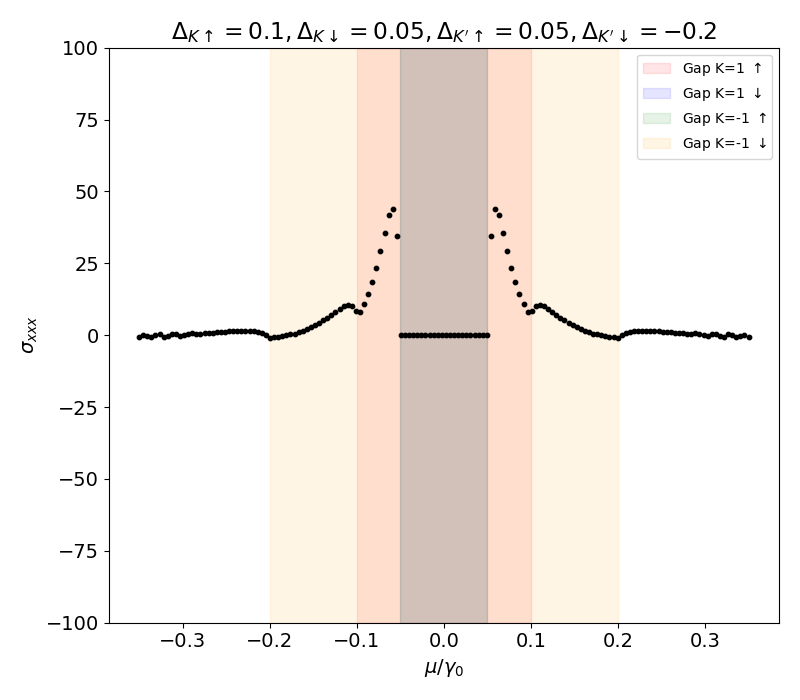
\includegraphics[width=0.7\textwidth]{../figures/scan_mu_PS_D_limited.png}
%     \caption{Nonlinear conductivity for asymmetric gaps with non-zero minor gaps (Zoomed to [-100, 100]).}
%     \label{fig:scan_D_lim}
% \end{figure}


\end{document}
